\section{Domain Analysis}

\subsection{Objective of the Laboratory Work}

The objective of this laboratory work is to design and implement a modular dual-actuator control system on an Arduino Mega 2560 microcontroller. The system controls two types of actuators --- a binary actuator (relay) and an analog actuator (PWM-driven motor/LED) --- through serial commands, with real-time signal conditioning and status reporting on an LCD display.

This lab addresses Varianta C of the assignment (100\% score), which requires simultaneous control of both a binary and an analog actuator, each with dedicated signal conditioning pipelines and unified display reporting. The key learning objectives include understanding the principles of actuator control in embedded systems, implementing counter-based debouncing for binary signals, applying ramping and filtering techniques for smooth analog control, and coordinating multiple real-time tasks using FreeRTOS.

\subsection{Problem Definition}

\begin{quote}
\textit{(Original task statement in Romanian --- Section 5.2 from the lab manual)}

Pentru un actuator binar bec iluminare prin releu, sau altul convenit cu mentorul s\u{a} se realizeze o aplica\c{t}ie pentru MCU care va interpreata comenzi de control de la utilizator prin STDIO (serial sau keypad), va controla actuatorul afi\c{s}\^{a}nd starea curent\u{a} pe un display LCD.

Varianta C: Implementarea sistem de control a doi actuatori, unul binar \c{s}i unul analogic, cu afi\c{s}area valorilor \c{s}i alertelor de la ambii actuatori pe display LCD.
\end{quote}

The task requires the development of a microcontroller application with the following capabilities:

\begin{enumerate}
    \item \textbf{Binary actuator control:} receive ON/OFF commands from the serial terminal, apply counter-based debouncing to prevent false switching, and drive a relay module that controls an external load (simulated lamp).
    \item \textbf{Analog actuator control:} receive speed commands (0--100\%) from the serial terminal, apply ramping for smooth transitions and signal conditioning (saturation, median filtering, EWMA) to eliminate noise, and drive a PWM output controlling a motor or LED.
    \item \textbf{Display and reporting:} periodically display the state of both actuators on a 16x2 LCD and print structured reports to the serial terminal, including debounce counters and conditioning diagnostics.
    \item \textbf{Multi-task architecture:} use FreeRTOS to run command parsing, binary control, analog control, and display as independent tasks with protected shared state via mutex.
\end{enumerate}

\subsection{Technical Requirements}

\subsubsection{Functional Requirements}

\begin{enumerate}
    \item[FR1] The system shall accept \texttt{ON} and \texttt{OFF} commands to control the binary actuator (relay).
    \item[FR2] The system shall accept \texttt{SPEED N} commands (N = 0--100) to set the analog actuator duty cycle.
    \item[FR3] The system shall accept a \texttt{STATUS} command to query the current state of both actuators.
    \item[FR4] The binary actuator command shall pass through a counter-based debounce filter (5 confirmations at 100\,ms intervals) before the relay state changes.
    \item[FR5] The analog actuator setpoint shall be ramped at a maximum rate of 5\%/cycle and processed through a signal conditioning pipeline (saturation 0--100\%, median filter, EWMA).
    \item[FR6] The LCD shall display the relay state, PWM duty cycle, debounce counter, and raw setpoint, updated every 500\,ms.
    \item[FR7] A serial report with both actuator states and conditioning diagnostics shall be printed every 500\,ms.
\end{enumerate}

\subsubsection{Non-Functional Requirements}

\begin{enumerate}
    \item[NFR1] The system shall respond to serial commands with a latency below 100\,ms.
    \item[NFR2] All shared variables between FreeRTOS tasks shall be protected by a mutex to prevent data races.
    \item[NFR3] The software shall be modular, with separate library modules for each hardware driver and signal conditioner.
    \item[NFR4] Pin assignments shall be defined in a single configuration header for consistency across code, simulation, and documentation.
\end{enumerate}

\subsection{Test Scenarios and Validation Criteria}

\begin{enumerate}
    \item \textbf{TC1 --- Binary ON command:} send ``ON'' via serial. Expected: after 5 debounce cycles (500\,ms), relay activates, green LED turns on, LCD shows ``Rly:ON''.
    \item \textbf{TC2 --- Binary OFF command:} send ``OFF'' after relay is ON. Expected: after 5 debounce cycles, relay deactivates, green LED turns off.
    \item \textbf{TC3 --- Rapid toggle rejection:} send ``ON'' then immediately ``OFF'' before debounce completes. Expected: relay state does not change (debounce counter resets).
    \item \textbf{TC4 --- Analog speed command:} send ``SPEED 75''. Expected: PWM ramps gradually to 75\%, signal conditioning smooths the transition, yellow LED turns on.
    \item \textbf{TC5 --- Analog ramp verification:} send ``SPEED 100'' from 0\%. Expected: duty increases by at most 5\%/cycle (100\,ms), reaching 100\% in approximately 2 seconds.
    \item \textbf{TC6 --- Analog saturation:} send ``SPEED 150''. Expected: duty clamped to 100\%.
    \item \textbf{TC7 --- Status command:} send ``STATUS''. Expected: serial prints current relay state and PWM duty cycle.
    \item \textbf{TC8 --- LCD display:} observe LCD during operation. Expected: line 1 shows relay state and PWM percentage, line 2 shows debounce counter and raw setpoint.
    \item \textbf{TC9 --- Unknown command:} send ``BLINK''. Expected: serial prints error message with usage help.
    \item \textbf{TC10 --- Dual actuator simultaneous:} send ``ON'' and ``SPEED 50'' in sequence. Expected: both actuators operate independently and are displayed on LCD.
\end{enumerate}

\subsection{Used Technologies}

\subsubsection{Actuator Control in Embedded Systems}

Actuators are devices that convert electrical energy into physical action. In embedded systems, actuators are the output stage that bridges the digital world of the microcontroller with the physical environment. They are broadly classified into two categories based on their control signal: binary actuators and analog actuators.

Binary actuators operate in only two states --- ON and OFF. The most common example is a relay, which is an electrically operated switch that uses an electromagnetic coil to mechanically open or close a circuit. Relays are widely used to control high-power loads (lamps, heaters, motors) from low-power microcontroller outputs. The relay coil typically requires more current than a GPIO pin can provide, so a transistor driver or dedicated relay module with an optocoupler is used for isolation and signal amplification. A critical consideration when controlling binary actuators is signal debouncing: commands arriving from noisy inputs (buttons, serial interface with potential repeated transmissions) must be validated through persistent confirmation before the actuator state is changed, preventing false switching that could damage equipment or create hazardous conditions.

Analog actuators accept a continuously variable control signal, allowing proportional control of physical quantities such as speed, position, brightness, or temperature. In microcontroller systems, the most common method for driving analog actuators is Pulse Width Modulation (PWM). PWM generates a square wave at a fixed frequency, and the duty cycle (the fraction of the period during which the signal is HIGH) determines the average power delivered to the actuator. For a DC motor, varying the duty cycle controls the speed; for an LED, it controls brightness. The relationship between duty cycle and average voltage is given by $V_{avg} = D \times V_{supply}$, where $D$ is the duty cycle (0.0 to 1.0). Signal conditioning for analog actuators includes saturation (clamping values to safe limits), filtering (removing noise from the command signal), and ramping (limiting the rate of change to prevent mechanical shock or current surges during rapid transitions).

\subsubsection{Counter-Based Debouncing}

Counter-based debouncing is a software technique for filtering noisy binary signals. Instead of accepting a state change immediately, the algorithm maintains a counter that increments when the input is HIGH and decrements when LOW. The output only transitions to ON when the counter reaches a maximum threshold, and to OFF when it reaches zero. Intermediate counter values retain the previous stable state. This approach is more robust than simple time-based debouncing because it can reject short bursts of noise while still responding quickly to sustained state changes. The number of required confirmations and the sampling interval together determine the minimum pulse duration that the filter will pass.

\subsubsection{Signal Conditioning for Analog Actuators}

The signal conditioning pipeline for analog actuator commands applies three sequential stages to the raw command value. First, saturation clamps the value to the physically valid range (0--100\% for a duty cycle), rejecting out-of-range commands. Second, a median filter removes impulsive noise by selecting the median from a sliding window of recent samples, effectively eliminating outlier values without distorting the signal shape. Third, an Exponentially Weighted Moving Average (EWMA) smooths the median-filtered value, reducing residual fluctuations while preserving responsiveness. Before entering this pipeline, a ramping stage limits the rate of change per control cycle, ensuring that the actuator transitions smoothly between setpoints.

\subsubsection{FreeRTOS Real-Time Operating System}

FreeRTOS is a real-time operating system kernel designed for microcontrollers and small embedded systems. It provides preemptive multitasking with priority-based scheduling, allowing multiple independent tasks to run concurrently on a single processor. Each task has its own stack and execution context, and the scheduler switches between tasks based on priority and timing constraints. FreeRTOS provides synchronization primitives such as mutexes and semaphores for protecting shared resources between tasks. In this lab, a mutex protects the shared command targets and actuator state variables that are written by the command task and read by the actuator and display tasks.

\subsubsection{PlatformIO Build System}

PlatformIO is a professional open-source ecosystem for embedded development. It provides project management, library dependency resolution, multi-board support, and integrated build/upload/monitor tools. In this lab, PlatformIO is used within VS Code to compile, upload, and monitor the application on the Arduino Mega 2560.

\subsubsection{Wokwi Simulator}

Wokwi is an online and VS Code-integrated simulator for embedded systems that supports Arduino, ESP32, and other popular platforms. It allows testing of the application in a virtual environment before deploying to physical hardware, providing a simulated serial terminal, virtual LEDs, relay modules, and I2C LCD displays.

\begin{figure}[H]
\centering
\IfFileExists{resources/DomainAnalysis/SoftwareComponents/wokwi.png}{%
    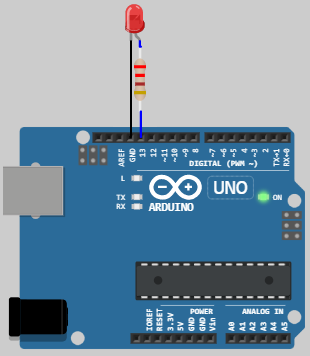
\includegraphics[width=0.6\textwidth]{resources/DomainAnalysis/SoftwareComponents/wokwi.png}%
}{%
    \fbox{\parbox{0.58\textwidth}{\centering\color{gray}\small
        [Screenshot pending --- save to resources/DomainAnalysis/SoftwareComponents/wokwi.png]}}%
}
\caption{Wokwi simulator interface for embedded circuit simulation}
\label{fig:wokwi_simulation}
\end{figure}

\subsection{Hardware Components}

\subsubsection{Arduino Mega 2560}

The Arduino Mega 2560 is a microcontroller development board based on the ATmega2560 AVR chip. It features 54 digital I/O pins (15 of which support PWM output), 16 analog inputs, 4 hardware UART ports, a 16\,MHz crystal oscillator, and USB connectivity. The board operates at 5\,V with 8\,KB SRAM and 256\,KB flash memory. In this lab, the Mega 2560 serves as the central controller, running FreeRTOS tasks that manage command parsing, actuator control, and display reporting.

\begin{figure}[H]
\centering
\IfFileExists{resources/DomainAnalysis/HardwareComponents/arduino_mega_2560.png}{%
    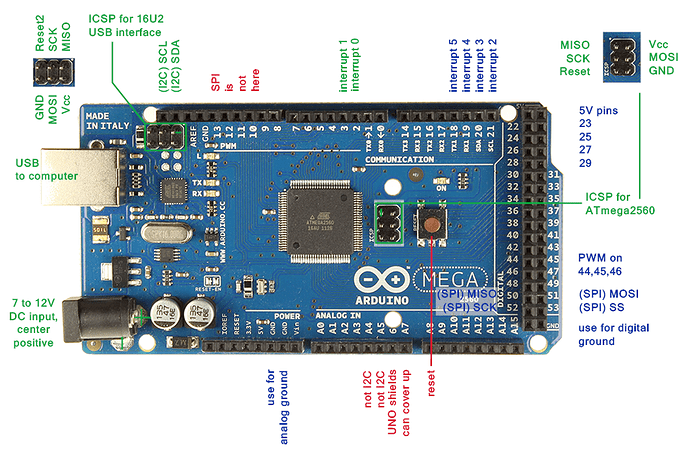
\includegraphics[width=0.7\textwidth]{resources/DomainAnalysis/HardwareComponents/arduino_mega_2560.png}%
}{%
    \fbox{\parbox{0.68\textwidth}{\centering\color{gray}\small
        [Image pending --- save to resources/DomainAnalysis/HardwareComponents/arduino\_mega\_2560.png]}}%
}
\caption{Arduino Mega 2560 development board}
\label{fig:arduino_mega}
\end{figure}

\subsubsection{Relay Module}

The relay module is a single-channel electromechanical switch controlled by a digital GPIO pin. It uses an optocoupler for electrical isolation between the microcontroller and the relay coil, and includes a flyback diode for coil spike protection. The module has three output terminals: COM (common), NO (normally open), and NC (normally closed). When the control pin is driven HIGH, the relay coil energizes and the COM-NO circuit closes, allowing current to flow through the external load. When driven LOW, the relay deactivates and COM-NO opens.

In this lab, the relay module is connected to pin 7 of the Arduino Mega 2560 and controls a simulated lamp (LED in Wokwi). The relay operates at 5\,V with a coil current of approximately 70\,mA, drawn from the board's 5\,V supply through the module's built-in driver circuit.

\begin{figure}[H]
\centering
\IfFileExists{resources/DomainAnalysis/HardwareComponents/relay_module.png}{%
    
\includegraphics[width=0.4\textwidth]{resources/DomainAnalysis/HardwareComponents/relay_module.png}%
}{%
    \fbox{\parbox{0.38\textwidth}{\centering\color{gray}\small
        [Image pending --- save to resources/DomainAnalysis/HardwareComponents/relay\_module.png]}}%
}
\caption{Single-channel relay module with optocoupler isolation}
\label{fig:relay_module}
\end{figure}

\subsubsection{LEDs and Resistors}

Three LEDs are used in this lab for status indication and load simulation. A green LED on pin 12 mirrors the relay state (ON when relay is active), providing visual feedback for the binary actuator. A yellow LED on pin 11 indicates analog actuator activity (ON when duty cycle exceeds 1\%). A blue LED on pin 9 (PWM-capable) simulates the analog actuator load --- in a physical system, this would be replaced by a DC motor with an appropriate driver circuit. Each LED is connected through a 220\,$\Omega$ current-limiting resistor to keep the forward current within safe limits ($I \approx 13.6$\,mA at 5\,V).

\begin{figure}[H]
\centering
\IfFileExists{resources/DomainAnalysis/HardwareComponents/led.png}{%
    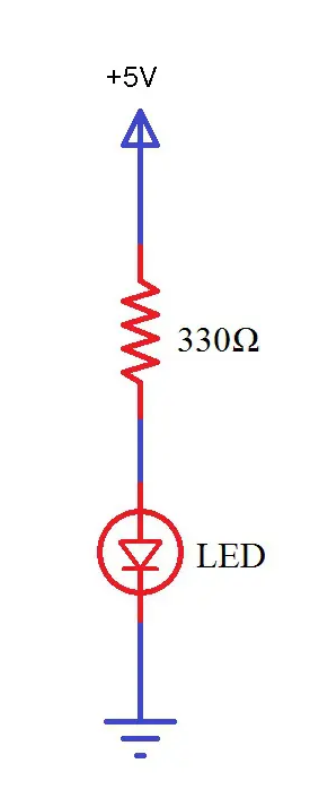
\includegraphics[width=0.15\textwidth]{resources/DomainAnalysis/HardwareComponents/led.png}%
}{%
    \fbox{\parbox{0.13\textwidth}{\centering\color{gray}\small
        [Image pending]}}%
}
\caption{Standard 5mm LED used as status indicator}
\label{fig:led_component}
\end{figure}

\subsubsection{LCD 1602 I2C Display}

The LCD 1602 is a 16-column, 2-row character display that communicates with the microcontroller over the I2C bus (address 0x27). An I2C backpack module reduces the required connections from 16 parallel pins to just 4 wires (VCC, GND, SDA, SCL). The display is connected to the Arduino Mega's I2C pins (SDA on pin 20, SCL on pin 21) and is used to show real-time status of both actuators, including relay state, PWM duty cycle, debounce counter, and raw setpoint.

\begin{figure}[H]
\centering
\IfFileExists{resources/DomainAnalysis/HardwareComponents/lcd_1602_i2c.png}{%
    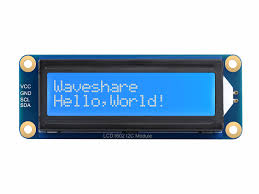
\includegraphics[width=0.4\textwidth]{resources/DomainAnalysis/HardwareComponents/lcd_1602_i2c.png}%
}{%
    \fbox{\parbox{0.38\textwidth}{\centering\color{gray}\small
        [Image pending --- save to resources/DomainAnalysis/HardwareComponents/lcd\_1602\_i2c.png]}}%
}
\caption{LCD 1602 display with I2C backpack module}
\label{fig:lcd_1602}
\end{figure}

\subsection{Software Components}

\subsubsection{Visual Studio Code with PlatformIO}

Visual Studio Code with the PlatformIO IDE extension provides the complete development environment for this project. PlatformIO handles project configuration via \texttt{platformio.ini}, automatic toolchain management for the AVR target, library dependency resolution (FreeRTOS, LiquidCrystal\_I2C), and integrated serial monitoring for testing commands and viewing reports.

\begin{figure}[H]
\centering
\IfFileExists{resources/DomainAnalysis/SoftwareComponents/platformio.png}{%
    
\includegraphics[width=0.6\textwidth]{resources/DomainAnalysis/SoftwareComponents/platformio.png}%
}{%
    \fbox{\parbox{0.58\textwidth}{\centering\color{gray}\small
        [Screenshot pending --- save to resources/DomainAnalysis/SoftwareComponents/platformio.png]}}%
}
\caption{PlatformIO IDE extension in Visual Studio Code}
\label{fig:platformio_extension}
\end{figure}

\subsection{System Architecture and Justification}

The system employs a layered software architecture combined with a FreeRTOS multi-task design. The architecture separates hardware drivers (relay, PWM, LED, LCD) from signal conditioning logic (debouncing, ramping, filtering) and application-level task orchestration.

The choice of FreeRTOS over the bare-metal TaskScheduler used in earlier labs is justified by the need for mutex-protected shared state between the command parser and actuator tasks. FreeRTOS provides preemptive scheduling with configurable task priorities, ensuring that the command parsing task (highest priority) can interrupt lower-priority display updates to maintain responsive command handling within the 100\,ms latency requirement.

The signal conditioning approach is tailored to each actuator type. For the binary actuator, counter-based debouncing (5 confirmations at 100\,ms intervals = 500\,ms minimum transition time) prevents false switching while remaining responsive to sustained commands. For the analog actuator, the combination of ramping (5\%/cycle rate limit) and the three-stage conditioning pipeline (saturation, median, EWMA) provides smooth, stable control that protects mechanical actuators from sudden load changes.

\subsection{Case Study: Industrial Relay Control Systems}

Relay-based control systems are ubiquitous in industrial automation. HVAC (Heating, Ventilation, and Air Conditioning) systems use relays to switch compressors, fans, and heating elements based on thermostat signals. Manufacturing production lines employ relay logic for sequencing conveyor belts, pneumatic actuators, and safety interlocks. Building management systems use relays to control lighting circuits, access gates, and fire suppression systems.

In all these applications, signal conditioning and debouncing are critical safety requirements. A false relay activation in an industrial oven or a medical sterilizer could cause overheating, while a false deactivation in a safety interlock could expose workers to hazardous conditions. The counter-based debouncing technique implemented in this lab mirrors the approach used in industrial programmable logic controllers (PLCs), where input filters with configurable persistence thresholds are standard practice for ensuring reliable actuator control.
